\documentclass{article}
\usepackage[frenchb]{babel}
\usepackage{amsfonts}
\usepackage{amsmath}
\usepackage[T1]{fontenc}
\usepackage[utf8]{inputenc}
\usepackage{amsthm}
\usepackage{graphicx}
\usepackage{subfigure}
\usepackage{hyperref}



\title{Apprentissage Statistique en Génomique}
\author{Dell'Aiera Clément, Prévosteau Clément}
\date{}

\newtheorem{definition}{Def}
\newtheorem{thm}{Théorème}
\newtheorem{ex}{Exercice}
\newtheorem{lem}{Lemme}
\newtheorem{dem}{Preuve}
\newtheorem{prop}{Proposition}
\newtheorem{cor}{Corollaire}

\newcommand{\Z}{\mathbb Z}
\newcommand{\R}{\mathbb R}
\newcommand{\C}{\mathbb C}
\newcommand{\Hil}{\mathcal H}
\newcommand{\Mn}{\mathcal M _n (\mathbb C)}

\begin{document}
\maketitle

\begin{abstract}
Dans ce document, nous présentons une application des méthodes apprises au cours donné par Jean-Philippe Vert intitulé \textit{Machine Learning for Computational Statistics}. Il s'agit d'extraire un profil génétique à partir des niveaux d'expression de 4654 gènes récoltés sur 184 individus qui ont ou n'ont pas rechuté après une chimiothérapie, profil dont le but est de savoir, étant donné les niveaux d'expression de ces gènes chez un patient, s'il risque de réchuter ou non, en vue d'adapter le traitement \textit{a priori}. 
\end{abstract}

\begin{figure}[!h]\centering
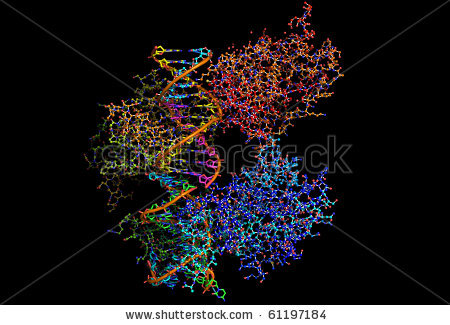
\includegraphics[scale=3]{dna.png}
\caption{A ball and stick model of molecules of protein p53 binding to a strand of DNA. The majority of human cancers involve mutations which make this protein inactive, from \url{http://fr.123rf.com/photo_7823791_.html}}
\label{fig:dna}
\end{figure}

\newpage

\tableofcontents

\newpage

\section{Support Vector Machine}

Nous avons entraîné des SVM sur la base d'apprentissage des $184$ patients initiaux, en faisant varier différents paramètres qu'offrait le package \textit{kernlab} sous \textit{R}. Par exemple, nous avons testé les noyaux : linéaires, gaussiens, Anova, TanH, Bessel et Laplace. A chaque fois, la marge a été déterminée par \textit{cross-validation} sur les $184$ patients, en divisant l'échantillon en $5$ classes.\\

Voici les marges optimales obtenues sur les 3 noyaux les plus efficaces, à savoir linéaires, gaussiens et Anova :
\begin{table}[!ht]
\center
\begin{tabular}{|c|c|}
\hline
\textbf{Noyau} & \textbf{Marge}\\
\hline
Linéaire & 0.0009765625\\
\hline
Gaussien & 0.125 \\
\hline
Anova & \\
\hline
\end{tabular}
\caption{Marges optimales des SVM obtenues par \textit{cross-validation}}
\label{Margin}
\end{table}

\begin{figure}[!h]\centering
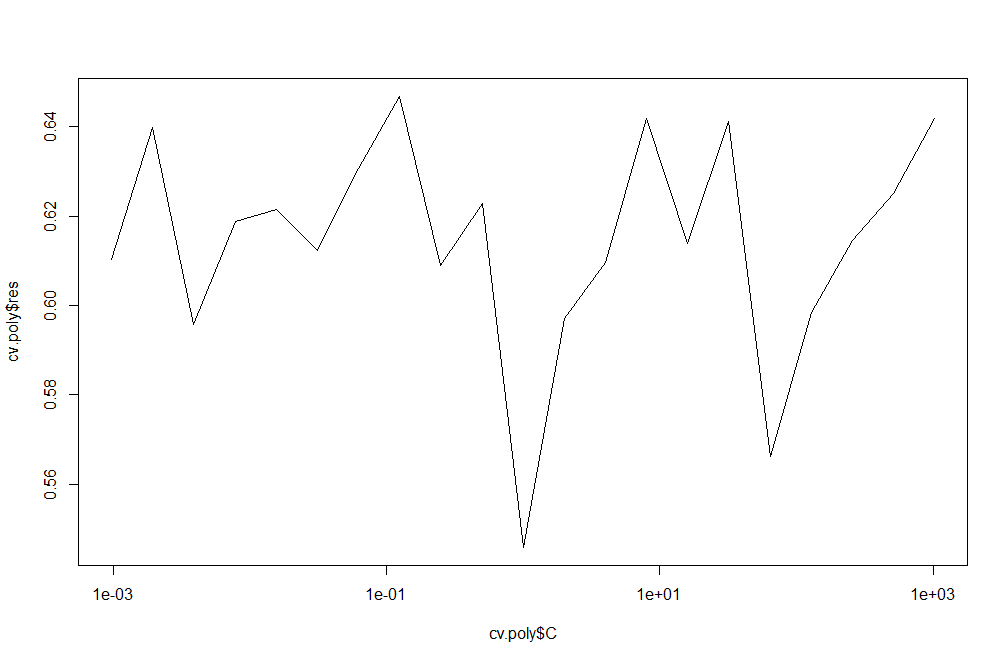
\includegraphics[scale=0.4]{auc.png}
\caption{Courbe de l'AUC pour un noyau polynomial de degré 2}
\label{fig:AUC Poly}
\end{figure}

L'échantillonage en $5$ sous-classes étant aléatoire, la marge$C$ obtenue varie à chaque itération. Afin d'obtenir un résultat plus robuste, nous avons itéré la cross-validation $100$ fois, puis fais la moyenne des marges optimales obtenues.\\

\subsection{Commentaires sur le code}
Nous avons principalement utilisé le package \textit{kernlab}.
Le code du projet est entièrement disponible à la page :\\

\url{https://github.com/cdellaie/MachineLearningforComputationalStat}

\subsection{Une mesure théorique de la connexité d'un graphe}
% a voir si cela peut servir , on peut le virer si ça sert vraiment à rien, je me suis dis que cela pouvait aider à choisir le nombre k des sous k graphe à choisir pour faire le group lasso

Voici la définition de la constante d'isopérimétrie d'un graphe. Provenant de la théorie des graphes expanseurs, elle mesure en quelque sorte, lorsque le graphe est fini, si le graphe est "très connexe", où l'on dit qu'un graphe est très connexe si, après lui avoir enlevé beaucoup d'arêtes, il le reste.\\

Si $X$ désigne un graphe fini, si $A\subset X$ est un sous-graphe de $X$, on définit la frontière de $A$ comme :
\[\partial A := \left\{(x,y)\ \text{arêtes t.q.} x\in A,y \notin A\right\}\]
Alors la constante d'isopérimétrie associée à $X$ est :
\[h(X)=\inf\left\{ \frac{|\partial A|}{|A|} : A \subset X \ \text{t.q.}\ 1\leq |A|\leq \frac{|X|}{2}\right\}\]
où $|.|$ dénote le cardinal d'un ensemble.

%linear subgraph
Un sous-graphe linéaire est constitué d'une suite de sommets qui forment un chemin, \textit{i.e.} une suite d'arêtes $v_j$ telles que $(v_j,v_{j+1})\in E$, où $E$ est l'ensemble des arêtes du graphe. 

%minimal connected component expected in the support of the model

\bibliographystyle{plain}
\bibliography{biblio} 

\end{document} 




































